\begin{enumerate}[label=\thesubsection.\arabic*,ref=\thesubsection.\theenumi]
	\item  Find the equation of the plane through the intersection of the planes $3{x} – {y} + 2{z} – 4 = 0 \text{ and } {x} + {y} + {z} – 2 = 0$ and the point $\myvec{2\\2\\1}$.
		\label{prob:12/11/3/9/plane}
		\\
    \solution
		\iffalse
\documentclass[journal,12pt,twocolumn]{IEEEtran}
\usepackage{setspace}
\usepackage{gensymb}
\usepackage{xcolor}
\usepackage{caption}
\singlespacing
\usepackage{siunitx}
\usepackage[cmex10]{amsmath}
\usepackage{mathtools}
\usepackage{hyperref}
\usepackage{amsthm}
\usepackage{mathrsfs}
\usepackage{txfonts}
\usepackage{stfloats}
\usepackage{cite}
\usepackage{cases}
\usepackage{subfig}
\usepackage{longtable}
\usepackage{multirow}
\usepackage{enumitem}
\usepackage{bm}
\usepackage{mathtools}
\usepackage{listings}
\usepackage{tikz}
\usetikzlibrary{shapes,arrows,positioning}
\usepackage{circuitikz}
\renewcommand{\vec}[1]{\boldsymbol{\mathbf{#1}}}
\DeclareMathOperator*{\Res}{Res}
\renewcommand\thesection{\arabic{section}}
\renewcommand\thesubsection{\thesection.\arabic{subsection}}
\renewcommand\thesubsubsection{\thesubsection.\arabic{subsubsection}}

\renewcommand\thesectiondis{\arabic{section}}
\renewcommand\thesubsectiondis{\thesectiondis.\arabic{subsection}}
\renewcommand\thesubsubsectiondis{\thesubsectiondis.\arabic{subsubsection}}
\hyphenation{op-tical net-works semi-conduc-tor}

\lstset{
language=Python,
frame=single, 
breaklines=true,
columns=fullflexible
}
\begin{document}
\theoremstyle{definition}
\newtheorem{theorem}{Theorem}[section]
\newtheorem{problem}{Problem}
\newtheorem{proposition}{Proposition}[section]
\newtheorem{lemma}{Lemma}[section]
\newtheorem{corollary}[theorem]{Corollary}
\newtheorem{example}{Example}[section]
\newtheorem{definition}{Definition}[section]
\newcommand{\BEQA}{\begin{eqnarray}}
        \newcommand{\EEQA}{\end{eqnarray}}
\newcommand{\define}{\stackrel{\triangle}{=}}
\newcommand{\myvec}[1]{\ensuremath{\begin{pmatrix}#1\end{pmatrix}}}
\newcommand{\mydet}[1]{\ensuremath{\begin{vmatrix}#1\end{vmatrix}}}
\bibliographystyle{IEEEtran}
\providecommand{\nCr}[2]{\,^{#1}C_{#2}} % nCr
\providecommand{\nPr}[2]{\,^{#1}P_{#2}} % nPr
\providecommand{\mbf}{\mathbf}
\providecommand{\pr}[1]{\ensuremath{\Pr\left(#1\right)}}
\providecommand{\qfunc}[1]{\ensuremath{Q\left(#1\right)}}
\providecommand{\sbrak}[1]{\ensuremath{{}\left[#1\right]}}
\providecommand{\lsbrak}[1]{\ensuremath{{}\left[#1\right.}}
\providecommand{\rsbrak}[1]{\ensuremath{{}\left.#1\right]}}
\providecommand{\brak}[1]{\ensuremath{\left(#1\right)}}
\providecommand{\lbrak}[1]{\ensuremath{\left(#1\right.}}
\providecommand{\rbrak}[1]{\ensuremath{\left.#1\right)}}
\providecommand{\cbrak}[1]{\ensuremath{\left\{#1\right\}}}
\providecommand{\lcbrak}[1]{\ensuremath{\left\{#1\right.}}
\providecommand{\rcbrak}[1]{\ensuremath{\left.#1\right\}}}
\theoremstyle{remark}
\newtheorem{rem}{Remark}
\newcommand{\sgn}{\mathop{\mathrm{sgn}}}
\newcommand{\rect}{\mathop{\mathrm{rect}}}
\newcommand{\sinc}{\mathop{\mathrm{sinc}}}
\providecommand{\abs}[1]{\left\vert#1\right\vert}
\providecommand{\res}[1]{\Res\displaylimits_{#1}}
\providecommand{\norm}[1]{\lVert#1\rVert}
\providecommand{\mtx}[1]{\mathbf{#1}}
\providecommand{\mean}[1]{E\left[ #1 \right]}
\providecommand{\fourier}{\overset{\mathcal{F}}{ \rightleftharpoons}}
\providecommand{\ztrans}{\overset{\mathcal{Z}}{ \rightleftharpoons}}
\providecommand{\system}[1]{\overset{\mathcal{#1}}{ \longleftrightarrow}}
\newcommand{\solution}{\noindent \textbf{Solution: }}
\providecommand{\dec}[2]{\ensuremath{\overset{#1}{\underset{#2}{\gtrless}}}}
\let\StandardTheFigure\thefigure
\def\putbox#1#2#3{\makebox[0in][l]{\makebox[#1][l]{}\raisebox{\baselineskip}[0in][0in]{\raisebox{#2}[0in][0in]{#3}}}}
\def\rightbox#1{\makebox[0in][r]{#1}}
\def\centbox#1{\makebox[0in]{#1}}
\def\topbox#1{\raisebox{-\baselineskip}[0in][0in]{#1}}
\def\midbox#1{\raisebox{-0.5\baselineskip}[0in][0in]{#1}}

\vspace{3cm}
\title{12.11.3.9}
\author{Lokesh Surana}
\maketitle
\section*{Class 12, Chapter 11, Exercise 3.9}


\solution The equation of given are given by
\begin{align}
	 {P}_1: \vec{n}_1^{\top}{\vec{x}} &= {c}_1\\
	 {P}_1: \vec{n}_1^{\top}{\vec{x}} &= {c}_2
\end{align}
%
\fi
The parameters of the given planes are
\begin{align}
 \vec{n}_1 = \myvec{3\\-1\\2},\,
 \vec{n}_1 = \myvec{1\\1\\1},\,
	c_1 = 4, c_2 = 2.
\end{align}
The intersection of the planes is given as
\begin{align}
\vec{n}_1^{\top}{\vec{x}} - {c}_1 + \lambda\brak{\vec{n}_2^{\top}{\vec{x}} - {c}_2} &= 0
\end{align}
where 
\begin{align}
	\lambda = \frac{{c}_1 - {n}_1^{\top}\vec{P}}{{n}_2^{\top}\vec{P} - {c}_2} 
= -\frac{2}{3}  
\end{align}
upon substituting 
\begin{align}
\vec{P} = \myvec{2\\2\\1}
\end{align}
Thus, 
the equation of plane is 
\begin{align}
 \myvec{7&-5&4}\vec{x} = 8
\end{align}


	\item  Find the equation of the line parallel to y-axis and drawn through the point of
intersection of the lines x – 7y + 5 = 0 and 3x + y = 0.
\\
\solution
		\iffalse
\documentclass[12pt]{article}
\usepackage{graphicx}
\usepackage{amsmath}
\usepackage{mathtools}
\usepackage{gensymb}
\usepackage[utf8]{inputenc}
\usepackage{float}
\newcommand{\mydet}[1]{\ensuremath{\begin{vmatrix}#1\end{vmatrix}}}
\providecommand{\brak}[1]{\ensuremath{\left(#1\right)}}
\providecommand{\norm}[1]{\left\lVert#1\right\rVert}
\newcommand{\solution}{\noindent \textbf{Solution: }}
\newcommand{\myvec}[1]{\ensuremath{\begin{pmatrix}#1\end{pmatrix}}}
\let\vec\mathbf

\begin{document}
\begin{center}
\textbf\large{CLASS-11 \\ CHAPTER-10 \\ STRAIGHT LINES}
\end{center}
\section*{Excercise 10.4}

\section*{Solution}
\fi
The given line can be expressed as
\begin{align}
\myvec{1&-7}\vec{x}&=-5\\
\myvec{3&1}\vec{x}&=0
\end{align}
The intersection of two lines is given by row reducing the augmented matrix
\begin{align}
\myvec{
1&-7&5\\
3&1&0
}
\xleftrightarrow[]{R_2=R_2-3R_1}
\myvec{
1&-7&5\\
0&22&-15
}\\\xleftrightarrow[]{R_2=\frac{R_2}{22}}
\myvec{
  1&-7&5\\[1pt]
0&1&-\frac{15}{22}
}
\xleftrightarrow[]{R_1={R_1}+7{R_2}}
\myvec{
1&0&\frac{5}{22}\\[1pt]
0&1&\frac{-15}{22}
}
\end{align}
yielding
\begin{align}
  \vec{P}&=\myvec{-\frac{5}{22}\\[1pt] \frac{15}{22}}
\end{align}
The normal vector of the desired 
line is 
\begin{equation}
    \vec{n}=\myvec{1\\0}
    \label{eq:chapters/11/10/4/6/normal}
\end{equation}
The desired equation is then given by 
\begin{align}
	\vec{n}^{\top}\myvec{\vec{x}-\vec{P}}&=0
	\\
\implies 
	\myvec{1&0}\vec{x}&=-\frac{5}{22}
\end{align}
See Fig. 
\ref{fig:chapters/11/10/4/6/Fig3}
\begin{figure}[!ht]
  \begin{center} 
      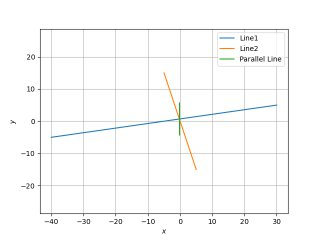
\includegraphics[width=\columnwidth]{chapters/11/10/4/6/figs/line_fig.png}
  \end{center}
\caption{}
\label{fig:chapters/11/10/4/6/Fig3}
\end{figure}

    \item A person standing at the junction (crossing) of two straight paths 
    represented by the equations 
    \begin{align}
        \myvec{2&-3}\vec{x} = -4 
        \label{eq:chapters/11/10/4/24/L1}
    \end{align}
    and
    \begin{align}
        \myvec{3&4}\vec{x} = 5
        \label{eq:chapters/11/10/4/24/L2}
    \end{align} 
    wants to reach the path whose equation is 
    \begin{align}
        \myvec{6&-7}\vec{x} = -8
        \label{eq:chapters/11/10/4/24/L3}
    \end{align}
    Find equation of the path that he should follow.
\\
    \solution 
		\iffalse
\documentclass[journal,12pt,twocolumn]{IEEEtran}
\usepackage{setspace}
\usepackage{gensymb}
\usepackage{xcolor}
\usepackage{caption}
\singlespacing
\usepackage{siunitx}
\usepackage[cmex10]{amsmath}
\usepackage{mathtools}
\usepackage{hyperref}
\usepackage{amsthm}
\usepackage{mathrsfs}
\usepackage{txfonts}
\usepackage{stfloats}
\usepackage{cite}
\usepackage{cases}
\usepackage{subfig}
\usepackage{longtable}
\usepackage{multirow}
\usepackage{enumitem}
\usepackage{mathtools}
\usepackage{listings}
\usepackage{tikz}
\usetikzlibrary{shapes,arrows,positioning}
\usepackage{circuitikz}
\let\vec\mathbf
\DeclareMathOperator*{\Res}{Res}
\renewcommand\thesection{\arabic{section}}
\renewcommand\thesubsection{\thesection.\arabic{subsection}}
\renewcommand\thesubsubsection{\thesubsection.\arabic{subsubsection}}

\renewcommand\thesectiondis{\arabic{section}}
\renewcommand\thesubsectiondis{\thesectiondis.\arabic{subsection}}
\renewcommand\thesubsubsectiondis{\thesubsectiondis.\arabic{subsubsection}}
\hyphenation{op-tical net-works semi-conduc-tor}

\lstset{
language=Python,
frame=single, 
breaklines=true,
columns=fullflexible
}
\begin{document}
\theoremstyle{definition}
\newtheorem{theorem}{Theorem}[section]
\newtheorem{problem}{Problem}
\newtheorem{proposition}{Proposition}[section]
\newtheorem{lemma}{Lemma}[section]
\newtheorem{corollary}[theorem]{Corollary}
\newtheorem{example}{Example}[section]
\newtheorem{definition}{Definition}[section]
\newcommand{\BEQA}{\begin{eqnarray}}
\newcommand{\EEQA}{\end{eqnarray}}
\newcommand{\define}{\stackrel{\triangle}{=}}
\newenvironment{amatrix}[1]{%
  \left(\begin{array}{@{}*{#1}{c}|c@{}}
}{%
  \end{array}\right)
}
\newcommand{\myvec}[1]{\ensuremath{\begin{pmatrix}#1\end{pmatrix}}}
\newcommand{\myaugvec}[2]{\ensuremath{\begin{amatrix}{#1}#2\end{amatrix}}}
\newcommand{\mydet}[1]{\ensuremath{\begin{vmatrix}#1\end{vmatrix}}}
\bibliographystyle{IEEEtran}
\providecommand{\nCr}[2]{\,^{#1}C_{#2}} % nCr
\providecommand{\nPr}[2]{\,^{#1}P_{#2}} % nPr
\providecommand{\mbf}{\mathbf}
\providecommand{\pr}[1]{\ensuremath{\Pr\left(#1\right)}}
\providecommand{\qfunc}[1]{\ensuremath{Q\left(#1\right)}}
\providecommand{\sbrak}[1]{\ensuremath{{}\left[#1\right]}}
\providecommand{\lsbrak}[1]{\ensuremath{{}\left[#1\right.}}
\providecommand{\rsbrak}[1]{\ensuremath{{}\left.#1\right]}}
\providecommand{\brak}[1]{\ensuremath{\left(#1\right)}}
\providecommand{\lbrak}[1]{\ensuremath{\left(#1\right.}}
\providecommand{\rbrak}[1]{\ensuremath{\left.#1\right)}}
\providecommand{\cbrak}[1]{\ensuremath{\left\{#1\right\}}}
\providecommand{\lcbrak}[1]{\ensuremath{\left\{#1\right.}}
\providecommand{\rcbrak}[1]{\ensuremath{\left.#1\right\}}}
\theoremstyle{remark}
\newtheorem{rem}{Remark}
\newcommand{\sgn}{\mathop{\mathrm{sgn}}}
\newcommand{\rect}{\mathop{\mathrm{rect}}}
\newcommand{\sinc}{\mathop{\mathrm{sinc}}}
\providecommand{\abs}[1]{\left\vert#1\right\vert}
\providecommand{\res}[1]{\Res\displaylimits_{#1}} 
\providecommand{\norm}[1]{\left\Vert#1\right\Vert}
\providecommand{\mtx}[1]{\mathbf{#1}}
\providecommand{\mean}[1]{E\left[ #1 \right]}
\providecommand{\fourier}{\overset{\mathcal{F}}{ \rightleftharpoons}}
\providecommand{\ztrans}{\overset{\mathcal{Z}}{ \rightleftharpoons}}
\providecommand{\system}[1]{\overset{\mathcal{#1}}{ \longleftrightarrow}}
\newcommand{\solution}{\noindent \textbf{Solution: }}
\providecommand{\dec}[2]{\ensuremath{\overset{#1}{\underset{#2}{\gtrless}}}}
\let\StandardTheFigure\thefigure
\def\putbox#1#2#3{\makebox[0in][l]{\makebox[#1][l]{}\raisebox{\baselineskip}[0in][0in]{\raisebox{#2}[0in][0in]{#3}}}}
     \def\rightbox#1{\makebox[0in][r]{#1}}
     \def\centbox#1{\makebox[0in]{#1}}
     \def\topbox#1{\raisebox{-\baselineskip}[0in][0in]{#1}}
     \def\midbox#1{\raisebox{-0.5\baselineskip}[0in][0in]{#1}}

\vspace{3cm}
\title{Line Assignment}
\author{Gautam Singh}
\maketitle
\bigskip

\begin{abstract}
    This document contains the solution to Question 24 of Exercise 4 
    in Chapter 10 of the class 11 NCERT textbook.
\end{abstract}

\begin{enumerate}
\fi
		We first find the coordinates of the intersection of \eqref{eq:chapters/11/10/4/24/L1}
    and \eqref{eq:chapters/11/10/4/24/L2}. Using the augmented matrix and row reduction methods,
    \begin{align}
        \myaugvec{2}{2&-3&-4\\3&4&5} &\xleftrightarrow[]{R_2\rightarrow2R_2-3R_1} 
        \myaugvec{2}{2&-3&-4\\0&17&22} \\
                      &\xleftrightarrow[]{R_1\rightarrow17R_1+3R_2} \myaugvec{2}{17&0&-1\\0&17&22} \\
                      &\xleftrightarrow[]{\substack{R_1\rightarrow\frac{R_1}{17}\\R_2\rightarrow\frac{R_2}{17}}} \myaugvec{2}{1&0&-\frac{1}{17}\\0&1&\frac{22}{17}}
        \label{eq:chapters/11/10/4/24/intersect}
    \end{align}
    the intersection of the lines is
    \begin{align}
        \vec{A} = \frac{1}{17}\myvec{-1\\22}
    \end{align}
    Clearly, the man should follow the path perpendicular to \eqref{eq:chapters/11/10/4/24/L3} from
    $\vec{A}$ to reach it in the shortest time. The normal vector 
    of \eqref{eq:chapters/11/10/4/24/L3} is 
    \begin{align}
        \vec{m} = \myvec{6\\-7}
        \label{eq:chapters/11/10/4/24/L3-norm}
    \end{align}
    which is consequently the direction vector of the required line. Therefore, 
    the required normal vector is given by
    \begin{align}
        \vec{n} = \myvec{7\\6}
        \label{eq:chapters/11/10/4/24/L4-norm}
    \end{align}
    and hence, the equation of the line is
   \begin{align}
        \vec{n}^\top\vec{x} &= \vec{n}^\top\vec{A} \\
        \implies \myvec{7&6}\vec{x} &= \frac{1}{17}\myvec{7&6}\myvec{-1\\22} = \frac{125}{17}
        \label{eq:chapters/11/10/4/24/L4}
    \end{align}
		See Fig. \ref{fig:chapters/11/10/4/24/crossing}. In this figure $\vec{F}$ represents 
    the foot of the prependicular drawn from $\vec{A}$ onto \eqref{eq:chapters/11/10/4/24/L3}.

	\item Find the equation of the line passing through the point of intersection of the lines $4x + 7y - 3 = 0$ and $2x - 3y + 1 = 0$ that has equal intercepts on the axes.\\
	\solution 
	  Given lines can be written in the form of \begin{align}
        \Vec{n}^{\top}\Vec{x} = c
    \end{align}
   Therefore,
		\begin{align}
       \myvec{4&7}\vec{x}=3
       \label{eq:11/10.4/12/2}
   \end{align} 
   \begin{align}
       \myvec{2&-3}\vec{x}=-1
       \label{eq:11/10.4/12/3}
   \end{align}
   Now, line equation that has equal intercepts on the axes is
   \begin{align}
       \myvec{1 & 1}\Vec{x}=c
       \label{eq:11/10.4/12/4}
   \end{align}
   Solving equations \eqref{eq:11/10.4/12/2} and \eqref{eq:11/10.4/12/3}
		augumented matrix is
 \begin{align}
    \myvec{4&7&3\\2&-3&-1}\\
    \xleftrightarrow{R_1 \leftarrow 4 R_1}
    \myvec{1&\frac{7}{4}&\frac{3}{4}\\2&-3&-1}
    \xleftrightarrow{R_2 \leftarrow R_2 - 2R_1}
    \myvec{1&\frac{7}{4}&\frac{3}{4}\\0&\frac{-13}{2}&\frac{-5}{2}}\\
    \xleftrightarrow{R_2 \leftarrow \frac{-2}{13}R_2}
    \myvec{1&\frac{7}{4}&\frac{3}{4}\\0&1&\frac{5}{13}}
    \xleftrightarrow{R_1 \leftarrow R_1-\frac{7}{4}R_2}
    \myvec{1&0&\frac{1}{13}\\0&1&\frac{5}{13}}
\end{align}
Therfore, \begin{align}    
\vec{x} = \myvec{\frac{1}{13}\\\frac{5}{13}}
\end{align}
Also this point lies on the equation \eqref{eq:11/10.4/12/4}
\begin{align}
    \myvec{1 & 1}\myvec{\frac{1}{13}\\\frac{5}{13}} = c\\
    \frac{1}{13}+\frac{5}{13} = c
    \end{align}
    Therefore, the equation is \begin{align}
        \myvec{1&1}\Vec{x}=\frac{6}{13}
    \end{align}

\item
Find the value of $p$ so that the three lines $3x+y-2=0, px+2y-3=0$ and $2x-y-3=0$ may intersect at one point.
\label{11.10.4.9}
\\
\solution
Performing row operations
on the matrix
\begin{align*}  
\myvec{
    3 &1&-2 \\
     p&2&-3\\
     2&-1&-3
}
\xrightarrow[R_3=3R_3-2R_1]{R_2=3R_2-pR_1}&\myvec{
    3&1&-2\\
     $0$&6-p&-9+2p\\
     0&-5&-5}\\
 \xrightarrow{R_3=R_3(6-p)+5R_2}&\myvec{
    3&1&-2\\
     0&6-p&-9+2p\\
     0&0&-75+15p}
     \\
  \implies 
    p=5
\end{align*}
Substituting this value in the above, we obtain
\begin{align}
\myvec{
    3&1&-2\\
     0&1&1\\
     0&0&0}
\end{align}
yielding
\begin{align}
	\vec{x} = \myvec{-1 \\ 1}
\end{align}
as the point of intersection.
    See \figref{fig:11.10.4.9}.
\begin{figure}[H]
    \centering
    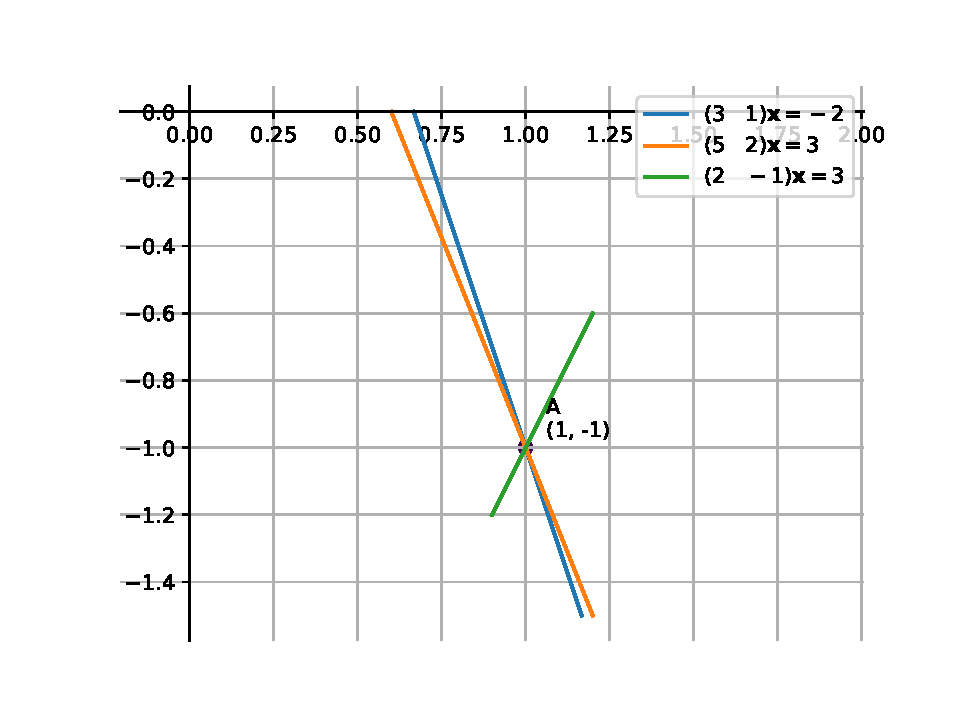
\includegraphics[width=0.75\columnwidth]{chapters/11/10/4/9/figs/fig.pdf}
    \caption{}
    \label{fig:11.10.4.9}
\end{figure}


\item Show the lines
$$\frac{x-1}{2}=\frac{y-2}{3}=\frac{z-3}{4}$$
$$\text{ and } \frac{x-4}{5}=\frac{y-1}{2}=z  \text{ intersect }.$$
 Also, find their point of intersection.
\item The area of the region bounded by the curve $y = x + 1$ and the lines $x = 2\text{ and }x = 3$ is
\begin{enumerate}
\item $\frac{7}{2}$ sq units
\item $\frac{9}{2}$ sq units
\item $\frac{11}{2}$ sq units
\item $\frac{13}{2}$ sq units
\end{enumerate}   
\item The area of the region bounded by the curve $x = 2 + 3$ and the $y$ lines $y = 1\text{ and }y = - 1$ is
\begin{enumerate}
\item 4 sq units 
\item $\frac{3}{2}$ sq units
\item 6 sq units
\item 8 sq units
\end{enumerate}
\item Compute the area bounded by the line $x + 2y = 2$, $y - x = 1\text{ and }2x + y = 7$.
\item Find the area bounded by the lines $y = 4x + 5$, $y = 5 - x\text{ and }4y = x + 5$.
\item Find the equation of the plane which is perpendicular to the plane $5x+3y+6z+8=0$ and which contains the line of intersection of the planes $x+2y+3z-4=0$ and $2x+y-z+5=0.$
\item  Point $\vec{P}(0,2)$ is the point of intersection of $y$-axis and perpendicular bisector of line segment joining the points $\vec{A}(-1,1) \text{ and } \vec{B}(3,3)$.
\item Prove that the line through A$(0,-1,-1)$ and B$(4,5,1)$ intersects the line through C$(3,9,4)$ and D$(-4,4,4)$.
\item Find the equation of the plane through the intersection of the planes $\overrightarrow{r} \cdot (\hat{i}+3\hat{j}) - 6=0$ and $\overrightarrow{r} \cdot (3\hat{i}-\hat{j}-4\hat{k})=0,$ whose perpendicular distance from origin is unity.
\item Find the equation of the line passing through the point of intersection of $2x+y=5\text{ and }x+3y+8=0$ and parallel the line $3x+4y=7$.
\item Find the equations of the lines through the point of intersection of the line $x-y+1=0 \text{ and }2x-3y+5=0$ and whose distance from the point (3,2) is $\frac{7}{5}$.
\item Equations of diagonals of the square formed by the lines $x=0$, $y=0$, $x=1$ and $y=1$ are
\begin{enumerate}
\item $y=x$, $y+x=1$
\item $y=x$,$x+y=2$
\item $2y=x$, $y+x=\frac{1}{3}$
\item $y=2x$, $y+2x=1$
\end{enumerate}
\item The straight line $5x+4y=0$ passes through the point of intersection of the straight lines $x+2y-10=0$ and $2x+y+5=0$.
\item Find the equation of the plane passing through the line of intersection of the planes  $\overrightarrow{r}\cdot(\hat{i}+\hat{j}+\hat{k})=1$ and $\overrightarrow{r}\cdot(2\hat{i}+3\hat{j}-\hat{k})+4=0$ and parallel to $x$-axis.
\item Find the equation of the plane which contains the line of intersection of the planes $\overrightarrow{r}\cdot(\hat{i}+2\hat{j}+3\hat{k})-4=0, \overrightarrow{r} \cdot  (2\hat{i}+\hat{j}-\hat{k})+5=0$ and which is perpendicular to the plane $\overrightarrow{r}\cdot(5\hat{i}+3\hat{j}-6\hat{k})+8=0$
\item Find the distance of the point $(-1,-5,-10)$ from the point of intersection of the line $\overrightarrow{r}=2\hat{i}-\hat{j}-2\hat{k}+\lambda(3\hat{i}+4\hat{j}+2\hat{k})$ and the plane $\overrightarrow{r}\cdot(\hat{i}-\hat{j}+\hat{k})=5$.
\end{enumerate}
